\begin{section}{Introduction}

Software development is a complex activity that demands the coordination of many people, such as programmers, designers, and managers. Software development activities should be coordinated in order to deliver products with high quality and on schedule. Many practices and processes have been proposed in order to aid the software development, targeting at high quality, low cost, fast delivery, or a combination of these.

Several researchers are concerned with the validity of studies based on bug tracking systems \cite{Aranda2009,Bird2009,Nguyen2010,Ayari2007}. The main concern is the accuracy of the information that is reported in such systems.
\end{section}

\begin{section}{Background}
\end{section}

  \begin{subsection}{Bug Tracking Systems}
Bug workflow. Bugzilla. \cite{Bird2009}

Reposit ́orios de bugs. Arquivam relat ́orios de defeitos e solicitac ̧ ̃oes de mudan ̧ca. Tais reposito ́rios ajudam os desenvolvedores a registrar, discutir e acompanhar a situa ̧ca ̃o de cada solicita ̧c ̃ao, desde a atribui ̧ca ̃o de uma solicita ̧ca ̃o a um desenvolvedor at ́e a verifica ̧c ̃ao da corre ̧c ̃ao ou melhoria. Exemplos incluem o Bugzilla, o Trac e o Jira.

Bug tracking systems are applications that allow users and developers of a software system to manage a list of bugs for the system. Usually, users and developers can report bugs, along with information such as steps to reproduce the bug and the operating system that was used. Then, developers choose bugs to fix and can report on the progress of the bug fixing activities, ask for clarification etc.

One important feature of a bug that is recorded on bug tracking systems is its status. The status records the progress of the bug fixing activity, and, as such, provides data to software engineering studies. Figure \ref{fig:bugzilla} shows each status that can be recorded in Bugzilla, a popular bug tracking system, along with typical transitions between statuses, i.e., the workflow. Other systems present comparable status and transitions.

\begin{figure}[ht]
	\centering
		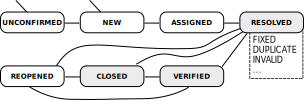
\includegraphics[scale=0.4]{bugzilla.png}
	\caption{Workflow for Bugzilla. Source: \url{http://www.bugzilla.org/docs/2.18/html/lifecycle.html}.}
	\label{fig:bugzilla}
\end{figure}

In the simplest cases, a bug is created and receive the status \texttt{UNCONFIRMED} or \texttt{NEW}. Next, it is assigned to a developer, and then it is resolved, possibly by fixing it with a patch on the source code. The solution is then verified by someone in the quality assurance team. If it passes the quality requirements, it is closed. If it doesn’t pass the quality requirements or if the solution only partially fixes the problem, the bug is reopened.
\end{subsection}

  \begin{subsection}{The Eclipse Project}
History. \\
Recommendations about Bugzilla usage. Four-eyes principle.

The Eclipse Project was created in 2001 by IBM and released into open source in 2004\footnote{\url{http://www.eclipse.org/org/}}, with focus on the creation of a extensible platform that supports the software development lifecycle. Today, it is maintained by its open source community, as well as by IBM employees and people from other organizations.

The Eclipse Project consists of many subprojects, including the Platform project and dozens of plugins. Although each subproject is maintained by a distinct team and is relatively autonomous, all of them should follow a general, documented process. 

All subprojects use Bugzilla for bug reporting, and there are clear rules regarding the process of change in the software\footnote{\url{http://wiki.eclipse.org/Development_Resources/HOWTO/Bugzilla_Use}}. Here is an excerpt of a document in the Eclipse web site that explains the bug fixing process\footnote{\url{http://wiki.eclipse.org/Bug_Reporting_FAQ}} (emphasis added):

\begin{quote}
When a new bug is entered it begins life with a Status of either \textbf{Unconfirmed} for normal users or \textbf{New} for users with commit privileges. The bug is typically assigned to the component owner. The component owner will usually use a query of Status = Unconfirmed or New and Assigned to = me to browse what is essentially the component's inbox. She or he will assign bug reports to developers. Email will be generated to the developer (this part is configurable). (Note that the act of reassigning a bug to somebody changes its status to New). The developer may change unconfirmed bugs to new.

The assigned developer will “accept” the bug which will change its status to \textbf{Assigned}. After working on the bug the developer will mark the bug as \textbf{Resolved} and will select a resolution (Fixed, Invalid, Wontfix, Worksforme).

Once a bug is resolved there are still a few states it can transition to. How you choose to use these states will be up to individual teams. In our example, when a test pass comes up a component owner can build a query that searched for resolved bugs. After testing that the fix worked a resolved bug can be transitioned to \textbf{verified}, directly to \textbf{closed}, or in fact, \textbf{reopened}. By searching for bugs with a Status of verified and a resolution of fixed developers can come up with release notes. A verified/fixed bug can then be transitioned to closed. And yes, closed bugs can be reopened if need be. As an added bonus other bug status can be transitioned through verified to closed as well. This gives developers the opportunity to test worksforme claims.
\end{quote}

There’s also a recommendation to follow the four eyes principle in the verification process (emphasis added):

\begin{quote}
When a developer fixes the bug, the status is set to RESOLVED - FIXED, and it is assigned to another developer on the team to verify. \textbf{It is important that the verifier be a different person than the fixer} because the fixer is too close to the code and thus may not be as diligent at testing the corner cases.
\end{quote}

Finally, there are additional guidelines regarding the workflow:

\begin{quote}
	\begin{itemize}
\item All bugs should be verified before the next integration build.

\item When a committer verifies a fix, the status is changed to VERIFIED.

\item When the project does a major release, the VERIFIED bugs are changed to CLOSED.
	\end{itemize}
\end{quote}
\end{subsection}

  \begin{subsection}{The Netbeans Project}
History. \\
Recommendations for developers.
\end{subsection}

\begin{section}{Experimental Setup}

\begin{verbatim}
Data extraction
Data processing: 
- filtering (bugs up to december 20xx)
- classification script
Sampling:
- random sampling (for coding)
- entire data set
Analysis:
- grounded theory (open coding)
- latent Dirichlet allocation
- descriptive statistics
\end{verbatim}

We have had access to Eclipse Bugzilla database from October, 2001 to June, 2010, in MySQL format. The data was made available as part of the Mining Software Repositories 2011 Challenge\footnote{\url{http://www.msrconf.org/msr-challenge.html}}.

The database includes data from 155 Eclipse subprojects. However, we have discarded subprojects in which no bug was ever reopened, and subprojects with less than 50 reported bugs.

For the remaining 34 subprojects, we have selected only bugs that were verified until December 2009. The rationale is that if, within six months, a verified bug was not reopened, it probably will not be reopened after that and it is, thus, fully fixed.
\end{section}

\begin{section}{Results}

	O que quer dizer “a solução de um bug foi verificada”?

	Como já foi comentado anteriormente, o Bugzilla permite que os relatórios de bugs sejam marcados como RESOLVED (resolvido) e, depois, como VERIFIED (verificado). Mas afinal, o que significa verificar a solução de um bug? Que atividades ou checagens foram realizadas antes de se marcar o bug como VERIFIED?

	A documentação do Bugzilla tem algo a dizer sobre isso o status VERIFIED:

	“QA [quality assurance team] has looked at the bug and the resolution and agrees that the appropriate resolution has been taken.”

	Essa definição sugere que a verificação deve ser feita por uma equipe especializada em controle de qualidade. Além disso, o verificador deve concordar que a resolução é apropriada. A definição do Bugzilla para por aí, mas eu consigo imaginar alguns critérios para considerar uma resolução apropriada:

	O bug não se manifesta após a aplicação da solução.
	A solução não gera novos bugs.
	O código da solução segue as convenções de codificação e políticas do projeto.
	A solução possui uma boa relação custo-benefício — isto é, ou não existem soluções melhores ou a solução é um paliativo por conta da alta complexidade de uma solução melhor.
	Minha expectativa, portanto, é que, antes de o bug ser marcado como VERIFICADO, ele passe pelas seguintes atividades:

	Aplicação do patch com a solução do bug na versão do software onde o bug foi encontrado.
	Execução do software com o bug, seguindo os passos para reprodução do bug, e verificando que o bug não se manifesta
	Inspeção do código-fonte. Deve ser verificada a aderência às convenções de codificação do projeto e a outras políticas (por exemplo, cada patch deve vir com testes de unidade).
	Execução de testes de unidade (se houver). Deve se verificar que todos os testes passam.
	Bom, mas isso é a teoria. Quais atividades são executadas na prática, em projetos reais, antes de se marcar um bug como VERIFIED? Para responder a essa pergunta, analisei um total de 80 bugs, considerando os projetos Eclipse/EMF, Eclipse/Platform, Netbeans/versioncontrol e Netbeans/profiler. Eis alguns casos verificados nesses projetos:

	O reporter (ou outro usuário que também enfrenta o problema) verificou que, em uma build do produto que inclui a solução, o bug deixou de se manifestar. Aparentemente não há inspeção do código-fonte, e nem uma equipe de QA. Situação frequente no Netbeans. Pode ser um procedimento necessário quando os desenvolvedores não conseguem reproduzir o bug.
	A solução está disponível em um build que é divulgado no site do projeto. Esse critério é usado pelo projeto Eclipse/EMF e foi decidido em reunião. O projeto usa o status FIXED para bugs cuja solução está no CVS.
	Bugs que já foram resolvidos há muito tempo são marcados como verificados, por se entender que, se nenhuma problema ocorreu até então, isso significa que a solução é adequada.
	A mesma pessoa que resolve o bug o marca como VERIFIED logo depois. Aparentemente não existe verificação de fato nesse caso.
	O desenvolvedor que resolve o bug solicita que outro desenvolvedor verifique a solução. Comum no Eclipse/Platform.
	No bug 249436 do Eclipse/EMF, um patch é submetido por um desenvolvedor, mas outro desenvolvedor acaba reescrevendo o patch, fornecendo evidências de que o código-fonte foi inspecionado.
	No bug 269789 do Eclipse/EMF, há evidências da elaboração e da execução de testes de unidade.
	A análise sugere que o status VERIFIED significa coisas diferentes em diferentes projetos. A execução de uma versão corrigida do software parece ser o método predominante de verificação. Em alguns casos, o status VERIFIED não representa verificação, e sim a indicação de que a solução está disponível para o usuário final. Evidências de inspeção de código e execução de testes de unidade só foram encontradas no projeto Eclipse/Platform.	

\end{section}

\begin{section}{Conclusion}
\end{section}

\section*{Acknowledgment}

The first author is supported by FAPESB under grant BOL0119/2010.
